\RequirePackage{flashmovie}
\documentclass[xcolor=table]{beamer}
%\documentclass{article}
\usepackage{amsmath}
\usepackage{xcolor}
\usepackage{animate}
%\usepackage{multimedia}
%\usepackage{movie15}
\DeclareMathOperator{\Bin}{Bin}
\setbeamertemplate{navigation symbols}{}
\setbeamertemplate{caption}{\insertcaption} \setbeamertemplate{caption label separator}{}
\renewcommand{\emph}{\textbf}
\usetheme{Warsaw}
\title{Ch. 3 -- Discrete Random Variables}
%\setlength{\parskip}{.2cm}

\begin{document}
\begin{frame}
\begin{beamercolorbox}[rounded=true,wd=\textwidth,center]{title}
\usebeamerfont{title}\inserttitle
\end{beamercolorbox}%\begin{center}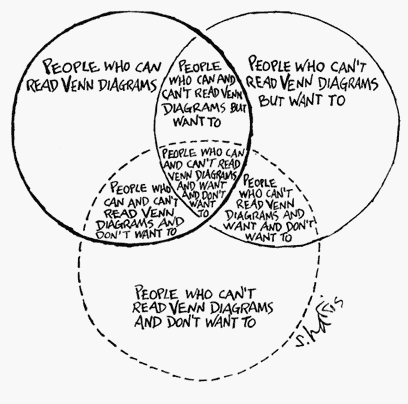
\includegraphics[scale=.4]{venn.png}
\vspace{1cm}
\begin{center}
\includegraphics[scale=.8]{galton.jpg}
\end{center}
\end{frame} 

\begin{frame}{Random Variables}
Given a set of outcomes $\Omega$, a \emph{random variable} is a number that depends on the outcome. A random variable is \emph{discrete} if its possible values can be listed in a sequence $x_1, x_2, \dots$

\pause \vspace{.5cm}
Example: Suppose we toss a fair coin 3 times. The set of outcomes is
$$\Omega=\{TTT,TTH,THT,THH,HTT,HTH,HHT,HHH\}$$
Let $X$ be the number of heads. Then $X$ is a random variable:

\begin{center}\begin{tabular}{p{4cm}p{4cm}}
\begin{tabular}{l}
$\begin{aligned}
TTT: X&=0 \\
TTH: X&=1 \\
THT: X&=1 \\
THH: X&=2
\end{aligned}$
\end{tabular} &
\begin{tabular}{l}
$\begin{aligned}
HTT: X&=1 \\
HTH: X&=2 \\
HHT: X&=2 \\
HHH: X&=3
\end{aligned}$
\end{tabular}
\end{tabular}
\end{center}

The possible values of $X$ are 0, 1, 2, and 3.
\end{frame}

\begin{frame}{Probability Mass Function}
In the previous example, we can calculate the probability of the number of heads $X$ being each of the values 0, 1, 2, and 3:
\begin{align*}
&P(X=0) = P(\{TTT\}) = 1/8 \\
&P(X=1) = P(\{HTT, THT, TTH \}) = 3/8 \\
&P(X=2) = P(\{HHT, HTH, THH\}) = 3/8 \\
&P(X=3) = P(\{HHH\}) = 1/8
\end{align*}
\pause The \emph{probability mass function} (pmf), $f(x)=P(X=x)$, describes the probability of each possible value:
\begin{center}
\begin{tabular}{p{6cm}p{6cm}}
\vspace{0cm}
\begin{tabular}{c||c|c|c|c}
x & 0 & 1 & 2 & 3 \\ \hline
f(x) & 1/8 & 3/8 & 3/8 & 1/8
\end{tabular}&
\vspace{-2cm}
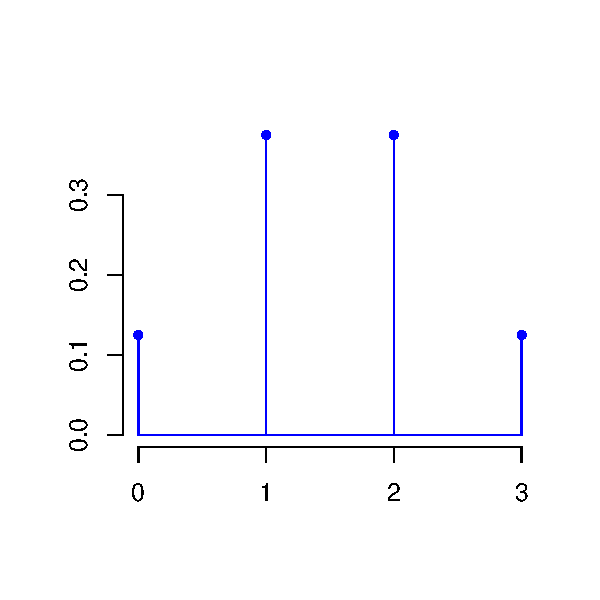
\includegraphics[scale=.5]{ch3_pmf.pdf}
\end{tabular}
\end{center}
\end{frame}


\begin{frame}{Sum of Two Random Variables}
Suppose we roll two six-sided dice, and let $X$ and $Y$ be the results. Their sum is a random variable $X+Y$ with values 2, 3, \dots, 12. What is the probability mass function of $X+Y$?

\pause\vspace{-.5cm}\begin{center}
\begin{tabular}{p{4.7cm}p{5.5cm}}
\vspace{0cm}
\begin{tabular}{l||p{.3cm}|p{.3cm}|p{.3cm}|p{.3cm}|p{.3cm}|p{.3cm}|}
& 1 & 2 & 3 & 4 & 5 & 6 \\ \hline \hline
1& 2 & 3 & 4 & 5 & 6 & 7 \\ \hline
2& 3 & 4 & 5 & 6 & 7 &  8  \\ \hline
3& 4 & 5 & 6 & 7 &  8 & 9 \\ \hline
4& 5 & 6 & 7 &  8 & 9 & 10\\ \hline
5& 6 & 7 &  8 & 9 &10 & 11\\ \hline
6& 7 &  8 & 9 & 10 & 11 & 12\\ \hline
\end{tabular}
&
\vspace{-1.5cm}
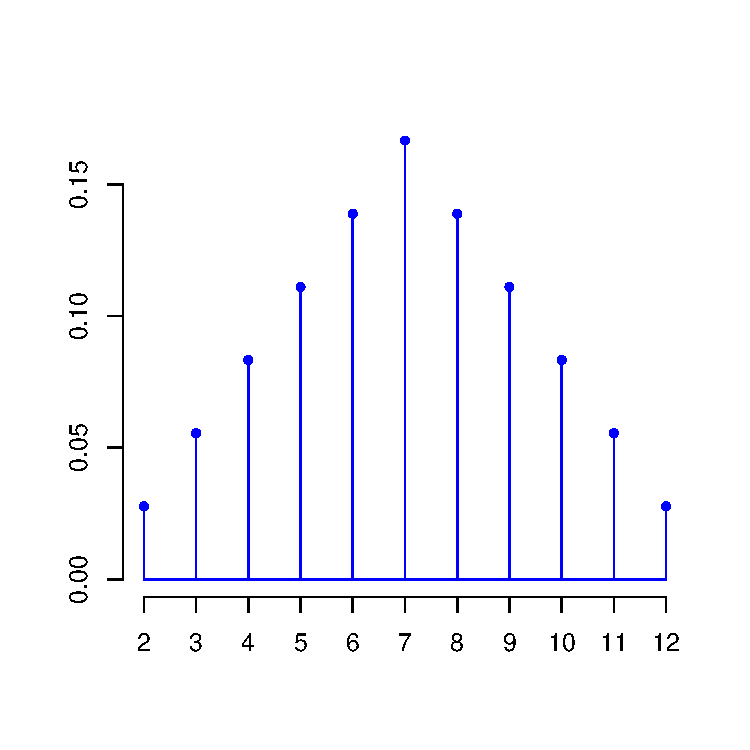
\includegraphics[scale=.5]{ch3_pmf2.pdf}
\end{tabular}

\vspace{-.5cm}
\renewcommand{\arraystretch}{1.5}
\begin{tabular}{c||c|c|c|c|c|c|c|c|c|c|c|}
$x$ & 2 & 3 & 4 & 5 & 6 & 7 & 8 & 9 & 10 & 11 & 12 \\ \hline
$f(x)$ & $\frac1{36}$ & $\frac2{36}$ & $\frac3{36}$ & $\frac4{36}$ & $\frac5{36}$ & $\frac6{36}$ & $\frac5{36}$ & $\frac4{36}$ & $\frac3{36}$ & $\frac2{36}$ & $\frac1{36}$
\end{tabular}
\end{center}
\end{frame}

\begin{frame}{Expected Value}
\begin{definition}
Given a discrete random variable $X$ with probability mass function $f(x)$, the \emph{expected value} of $X$ (or \emph{mean} of X) is
$$E(X) = \sum x\cdot f(x)$$ % = \sum x\cdot P(X=x)$$
where in the sum $x$ ranges over all possible values of $X$. For $E(X)$ we will sometimes write $\mu_X$ or just $\mu$.
\end{definition}

\pause Example: Recall that if we toss a fair coin three times, the number of heads $X$ has probability mass function
\begin{center}
\begin{tabular}{c||c|c|c|c}
x & 0 & 1 & 2 & 3 \\ \hline
f(x) & 1/8 & 3/8 & 3/8 & 1/8
\end{tabular}
\end{center}
The expected value of the number of heads is then
$$E(X) = \sum x\cdot f(x) = 0\cdot\frac18+1\cdot\frac38+2\cdot\frac38+3\cdot\frac18 = \frac{12}8 = 1.5$$
\end{frame}



\begin{frame}{Expected Value}
\begin{block}{}
If $X$ is a discrete random variable $X$ and $h(x)$ is a function, then $h(X)$ is also a discrete random variable, and
$$E[h(X)] =\sum h(x)\cdot f(x)$$
where $f(x)$ is the probability mass function of $X$.
\end{block}
\pause Example: Again let $X$ be the number of heads when tossing a fair coin 3 times. What is the expected value of $X^2$?

\pause\vspace{.3cm}
Recall the pmf of $X$:
%\begin{center}
\begin{tabular}{c||c|c|c|c}
x & 0 & 1 & 2 & 3 \\ \hline
f(x) & 1/8 & 3/8 & 3/8 & 1/8
\end{tabular}
%\end{center}

\vspace{.3cm}
Therefore, applying the formula above with $h(x)=x^2$,
\begin{align*}
E(X^2) &= \sum x^2 \cdot f(x) \\ 
&= 0^2\cdot\frac18+1^2\cdot\frac38+2^2\cdot\frac38+3^2\cdot\frac18 = \frac{24}8 = 3
\end{align*}
%\pause \vspace{.3cm}
%$X^2$ is a discrete random variable with possible values 0, 1, 4, and 9, with probabilities 1/8, 3/8, 3/8, and 1/8, respectively. Therefore,
%$$E(X^2) = 0\cdot\frac18+1\cdot\frac38+4\cdot\frac38+9\cdot\frac18 = \frac{24}8 = 3$$
\end{frame}


\begin{frame}{Properties of Expected Value}
\begin{block}{}
Let $X$ and $Y$ be random variables, and let $c$ be a constant. Then
\begin{enumerate}
\item $E(c) = c$
\item $E(cX) = cE(X)$
\item $E(X+Y) = E(X)+E(Y)$
%\item If $X$ and $Y$ are independent, then $E(XY) = E(X)E(Y)$.
\end{enumerate}
\end{block}

%\pause Example: If we toss a coin 3 times, the total number of heads $X$ may be expressed as the sum of the number of heads on each toss, $X=Y_1+Y_2+Y_3$, where $Y_1, Y_2, Y_3$ are independent Bernoulli random variables with parameter $p=.5$. Therefore,
%\begin{align*}
%E(X)& = E(Y_1+Y_2+Y_3)\\
%&= E(Y_1)+E(Y_2)+E(Y_3)\\
%&=.5+.5+.5= 1.5
%\end{align*}
\end{frame}

\begin{frame}{Example}
\begin{block}{}
Someone offers to let you play a game where you pay him \$10, toss a fair coin 3 times, and then he pays you back $3X+5$ dollars, where $X$ is the number of times the coin comes up heads.

\vspace{.3cm}
If you play, what is the expected amount of money that you will you be paid? On average, would this game work in your favor?
\end{block}

\pause
\vspace{.3cm}
Recall that if you toss a coin 3 times, the expected number of times the coin comes up heads is $E(X)=1.5$. \pause Therefore, using properties of expected value,
\begin{align*}
E(3X+5) &= E(3X)+E(5) \\
&= 3E(X)+5  \\
&= 3(1.5) + 5 = 9.5
\end{align*}
\pause So the expected payback is \$9.50. Since you have to pay \$10, this game would not work in your favor on average.
\end{frame}

%\begin{frame}{Properties of Expected Value}
%\begin{block}{}
%\vspace{-.2cm}$$E(c)=c$$
%\end{block}
%\pause Proof: A constant $X=c$ has only one possible value, $c$, and $P(X=c)=1$, so
%\pause \begin{align*}
%E(X) &= \sum_x x\cdot P(X=x) \\
%\uncover<4->{&= c \cdot P(X=c)} \\
%\uncover<5->{&= c\cdot 1} \\
%\uncover<6->{&= c}
%\end{align*}
%\end{frame}
%
%\begin{frame}{Properties of Expected Value}
%\begin{block}{}
%\vspace{-.2cm}$$E(cX)=cE(X)$$
%\end{block}
%
%\pause Proof: The possible values of $cX$ are just $c$ times the possible values of $X$, so
%\pause \begin{align*}
%E(cX) &= \sum_t t\cdot P(cX=t)\\
%\uncover<4->{&= \sum_x cx\cdot P(cX=cx) \\}
%\uncover<5->{&= \sum_x cx\cdot P(X=x)  \\}
%\uncover<6->{&= c\sum_x x\cdot P(X=x) \\}
%\uncover<7->{&= cE(X)}
%\end{align*}
%\end{frame}
%
%\begin{frame}{Properties of Expected Value}
%\vspace{-.15cm}\begin{block}{}
%\vspace{-.2cm}$$E(X+Y) = E(X)+E(Y)$$
%\end{block}
%\small
%\vspace{-.55cm}\pause \begin{align*}
%E(X+Y) &= \sum_t t\cdot P(X+Y=t) \\
%\uncover<3->{&=\sum_t t \sum_x \sum_y P(X=x, Y=y, X+Y=t) \\}
%%&=\sum_t \sum_x \sum_y t\cdot P(X=x, Y=y, X+Y=t) \\
%\uncover<4->{&=\sum_t \sum_x \sum_y (x+y)\cdot P(X=x, Y=y, X+Y=t) \\}
%\uncover<5->{&=\sum_x \sum_y  (x+y)\cdot P(X=x, Y=y) \\}
%\uncover<6->{&= \sum_x\sum_y x\cdot P(X=x, Y=y) + \sum_x\sum_y y\cdot P(X=x, Y=y) \\}
%\uncover<7->{&= \sum_x x\sum_y P(X=x, Y=y) + \sum_y y \sum_x P(X=x, Y=y) \\}
%\uncover<8->{&= \sum_x x\cdot P(X=x) + \sum_y y\cdot P(Y=y) \\}
%\uncover<9->{&= E(X)+E(Y)}
%\end{align*}
%\end{frame}
%
%\begin{frame}{Properties of Expected Value}
%\vspace{-.15cm}\begin{block}{}
%If $X$ and $Y$ are independent, then $E(XY)=E(X)E(Y)$.
%\end{block}
%\vspace{-.5cm}
%\pause \begin{align*}
%E(XY) &= \sum_t t\cdot P(XY=t) \\
%\uncover<3->{&= \sum_t \sum_x \sum_y t\cdot P(X=x, Y=y, XY=t) \\}
%\uncover<4->{&= \sum_t \sum_x \sum_y  xy \cdot P(X=x, Y=y, XY=t) \\}
%\uncover<5->{&= \sum_x \sum_y xy\cdot P(X=x, Y=y) \\}
%\uncover<6->{&= \sum_x \sum_y xy\cdot P(X=x)P(Y=y) \\}
%\uncover<7->{&= \left(\sum_x x\cdot P(X=x)\right) \left(\sum_y y\cdot P(Y=y)\right)\\}
%\uncover<8->{&= E(X)E(Y)}
%\end{align*}
%\end{frame}

\begin{frame}{Variance and Standard Deviation}
\vspace{-.1cm}
\begin{definition}
Given a discrete random variable $X$ with probability mass function $f(x)$ and mean $\mu=E(X)$, the \emph{variance} of $X$ is
$$V(X)=E[(X-\mu)^2]$$ %=\sum (x-\mu)^2\cdot f(x)$$
The variance of $X$ is sometimes written as $\sigma_X^2$ or just $\sigma^2$.
The \emph{standard deviation} of $X$ is the square root of the variance:
%$$\sigma = SD(X) = \sqrt{V(X)}$$
$$\sigma = \sqrt{V(X)}$$
\end{definition}

\pause Example: Again let $X$ be the number of heads when tossing a fair coin 3 times. We know that $\mu=E(X)=1.5$. What is $V(X)$?
\pause \begin{align*}
V(X)&=E[(X-\mu)^2] = \sum (x-\mu)^2 \cdot f(x) \\
&= (0-1.5)^2\cdot\frac18 + (1-1.5)^2\cdot\frac38+(2-1.5)^2\cdot\frac38+(3-1.5)^2\cdot\frac18\\
&= %\frac{2.25}8+\frac{0.75}8+\frac{0.75}8+\frac{2.25}8 = \frac68 = 
0.75
\end{align*}
\end{frame}

\begin{frame}{Shortcut Formula for Variance}
Let $X$ be a discrete random variable with mean $E(X)=\mu$. 
\begin{block}{}
\vspace{-.1cm}$$V(X) = E(X^2)-\mu^2$$
\end{block}

\pause
\vspace{.2cm}
Proof:\hspace{1cm}$\begin{aligned}[t]
V(X)&=E[(X-\mu)^2] \\
\uncover<3->{&= E(X^2 - 2\mu X+\mu^2) \\}
\uncover<4->{&= E(X^2) - 2\mu E(X)+E(\mu^2) \\}
\uncover<5->{&= E(X^2) - 2\mu^2 +\mu^2 = E(X^2)-\mu^2}
\end{aligned}$

\vspace{.3cm}
\uncover<6->{ Example: Again let $X$ be the number of heads when tossing a fair coin 3 times. We know that $\mu=E(X)=1.5$.} \uncover<7->{ Then}
\begin{align*}
\uncover<7->{V(X) &= E(X^2) - \mu^2\\}
\uncover<8->{&= \left(0^2\cdot\frac18 + 1^2\cdot\frac38 + 2^2\cdot\frac38+3^2\cdot\frac18\right) - 1.5^2\\}
\uncover<9->{&= 0.75}
\end{align*} 


%\uncover<6->{Example: 
%We can use the shortcut formula to rederive the variance of a Bernoulli random variable $X$ with parameter $p$.
%}
%
%\vspace{.2cm}\uncover<7->{ The only possible values of $X$ are 0 and 1, so $X^2=X$.} 
%\uncover<8->{
%\begin{align*}
%V(X)&=E(X^2)-[E(X)]^2 \\
%&= E(X)-[E(X)]^2= p-p^2= p(1-p)
%\end{align*}}
\end{frame}


\begin{frame}{Bernoulli Random Variable}
One of the simplest kinds of random variables is one which takes only two possible values: 0 and 1. We call $X$ a \emph{Bernoulli random variable} with parameter $p$ if
\begin{align*}
P(X=1)&= p \\
P(X=0)&= 1-p
\end{align*}

\pause\vspace{-1cm}
\begin{center}
\begin{tabular}{p{3cm}p{3cm}}
\begin{tabular}{c||c|c}
$x$ & 0 & 1 \\ \hline
$f(x)$ & 1-p & p
\end{tabular}
&
\begin{tabular}{c}
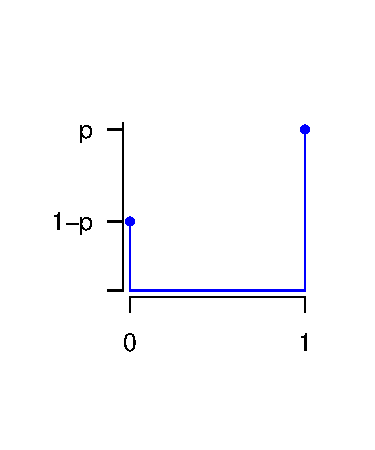
\includegraphics[scale=.5]{ch3_pmf3.pdf}
\end{tabular}
\end{tabular}
\end{center}

\pause\vspace{-1cm} For example, if we toss a fair coin, then the outcome is a Bernoulli random variable with parameter $p=1/2$, with 0 representing tails, and 1 representing heads.
\end{frame}


\begin{frame}{Mean and Variance of Bernoulli Random Variable}
Let $X$ be a Bernoulli random variable with parameter $p$. This means that the probability mass function (pmf) of $X$ is
\begin{center}
\begin{tabular}{c||c|c}
$x$ & 0 & 1 \\ \hline
$f(x)$ & 1-p & p
\end{tabular}
\end{center}
What is the expected value and variance of $X$?
\pause 
\begin{align*}
\mu &= E(X) = \sum x\cdot f(x) \\
&= 0\cdot (1-p) + 1\cdot p = p
\end{align*}

\vspace{-.5cm}
\pause
\begin{align*}
V(X) &= E((X-\mu)^2) = E((X-p)^2)\\
&= \sum (x-p)^2\cdot f(x)\\
&=(0-p)^2\cdot (1-p) + (1-p)^2\cdot p \\
&= p^2(1-p)+p(1-p)^2 \\
&= p(1-p)(p+(1-p)) = p(1-p)
\end{align*}
\end{frame}



\begin{frame}{Independent Random Variables}
Recall that two events $A$ and $B$ are independent if
$$P(A \cap B)=P(A)P(B)$$

\pause \begin{definition}
We say that discrete random variables $X$ and $Y$ are \emph{independent} if for any possible values $a$ and $b$ of $X$ and $Y$ respectively,
$$P(X=a \cap Y=b)=P(X=a)P(Y=b)$$
\end{definition}
\pause This definition generalizes to several random variables: We say that $X_1, X_2, X_3, \dots$ are \emph{independent} if for all $k$ and all possible values $a_1, a_2, a_3,\dots,a_k$ of $X_1, X_2, X_3, \dots,X_k$ respectively,
$$P(X_1=a_1 \cap \dots \cap X_k=a_k)=
P(X_1=a_1)\cdots P(X_k=a_k)$$
\end{frame}


\begin{frame}{Problem}
\begin{block}{}
Suppose that when we spin a coin, it only comes up heads with probability $.4$. If we spin the coin 3 times, find the probability mass function for the number of times we get heads.
\end{block}

\pause We may represent the outcomes of the three spins as independent Bernoulli random variables $Y_1$, $Y_2$, $Y_3$ each with parameter $.4$, where $Y_i=1$ if the $i$th spin is heads and $Y_i=0$ if the $i$th spin is tails. Then the number of heads is $X=Y_1+Y_2+Y_3$, \pause and
\begin{align*}
P(X=0)&=P(\{TTT\})\\
&=P(Y_1=0 \cap Y_2=0 \cap Y_3=0)\\
&= P(Y_1=0)P(Y_2=0)P(Y_3=0) \\
&= (.6)(.6)(.6) = .216
\end{align*}
\end{frame}

\begin{frame}
There are three ways to get heads exactly once:
\begin{align*}
P(X=1)&=P(\{HTT, THT, TTH\})\\
&= P(\{HTT\})+P(\{THT\})+P(\{TTH\})
\end{align*}
\pause We calculate,
\begin{align*}
P(\{HTT\})&=P(Y_1=1 \cap Y_2=0 \cap Y_3=0)\\
&= P(Y_1=1)P(Y_2=0)P(Y_3=0) \\
&= (.4)(.6)(.6) = .144
\end{align*}
\pause Similarly $P(\{THT\})=P(\{TTH\})=.144$. Therefore,
\begin{align*}
P(X=1) &= P(\{HTT\})+P(\{THT\})+P(\{TTH\})\\
&= 3P(\{HTT\}) = 3(.144)= .432
\end{align*}

\end{frame}

\begin{frame}
By the same kind of reasoning,
\begin{align*}
P(X=2)&=P(\{HHT,HTH,THH\}) \\
&= 3P(\{HHT\}) \\
&= 3P(Y_1=1)P(Y_2=1)P(Y_3=0) \\
&= 3(.4)(.4)(.6) = .288 \\[.5cm]
P(X=3)&=P(\{HHH\}) \\
&= P(Y_1=1)P(Y_2=1)P(Y_3=1) \\
&= (.4)(.4)(.4) = .064
\end{align*}
\end{frame}

\begin{frame}
Putting this together, we found
\begin{align*}
P(X=0)&=.216 \\
P(X=1)&=.432 \\
P(X=2)&= .288 \\
P(X=3)&= .064
\end{align*}
Therefore, the probability mass function for $X$ is 

\begin{tabular}{p{6cm}p{4cm}}
\vspace{1cm}
\begin{tabular}{c||c|c|c|c}
x & 0 & 1 & 2 & 3 \\ \hline
f(x) & .216 & .432 & .288 & .064
\end{tabular}
&
\vspace{-1cm}
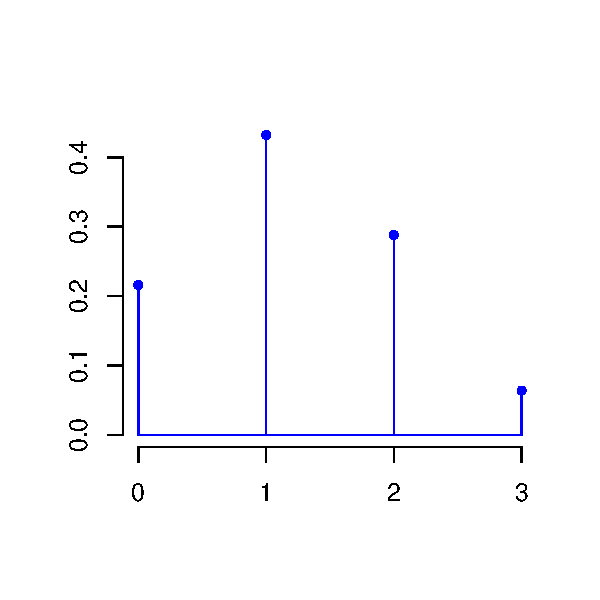
\includegraphics[scale=.5]{ch3_pmf5.pdf}
\vspace{-2cm}
\end{tabular}
\end{frame}

\begin{frame}{Binomial Distributions}
\begin{block}{}
Let $Y_1, Y_2, \dots, Y_n$ be independent Bernoulli random variables with parameter $p$. Then their sum
$$X=Y_1+Y_2+\cdots+Y_n$$
is a \emph{binomial random variable} with parameters $n$ and $p$. We write $X\sim \Bin(n,p)$
\end{block}
\pause In other words, given a sequence of $n$ independent trials, each with probability $p$ of success,  the binomial random variable $X$ counts the number of successes. The possible values of $X$ are 0, 1, \dots, $n$.

\vspace{.2cm}
\pause For example, if we toss a coin 3 times, then the number of heads $X$ is a binomial random variable with parameters $n=3$ and $p=.5$.
\end{frame}

\begin{frame}{Binomial Random Variables}
\begin{block}{}
If we toss a fair coin 4 times, what is the probability that we get exactly 2 heads?
\end{block}

\pause We may list the 16 equally likely outcomes:
\begin{center}\begin{tabular}{cccc}
TTTT & TTTH & TTHT & \cellcolor{cyan}TTHH \\
THTT & \cellcolor{cyan}THTH & \cellcolor{cyan}THHT & THHH \\
HTTT & \cellcolor{cyan}HTTH & \cellcolor{cyan}HTHT & HTHH \\
\cellcolor{cyan}HHTT & HHTH & HHHT & HHHH
\end{tabular}\end{center}
\pause Out of the 16 outcomes, 6 involve getting exactly 2 heads. Therefore,
$$P(X=2)=6/16=3/8 = .375$$
\pause However, it would be nice to be able to solve this without having to list all the outcomes.
\end{frame}

\begin{frame}{Counting}
\begin{block}{}
How many ways are there to rearrange the letters $ABCD$?
\end{block}
\pause \begin{center}\begin{tabular}{cccccc}
ABCD & ABDC & ACBD & ACDB & ADBC & ADCB \\
BACD & BADC & BCAD & BCDA & BDAC & BDCA \\
CABD & CADB & CBAD & CBDA & CDAB & CDBA \\
DABC & DACB & DBAC & DBCA & DCAB & DCBA
\end{tabular}\end{center}
\pause There are
\begin{align*}
&\text{ 4 choices for which letter to put in the first position}\\
\times & \text{ 3 choices for which letter to put in the second position}\\
\times & \text{ 2 choices for which letter to put in the third position}\\
\times & \text{ 1 choice for which letter to put in the fourth position}\\
= &\ 4\cdot 3\cdot2\cdot1 = 24
\end{align*}
\pause In general, the number of ways to rearrange $n$ distinct symbols is
$$n! = n(n-1)(n-2)\cdots3\cdot2\cdot1$$
\end{frame}

\begin{frame}{Counting}
\begin{block}{}
How many ways are there to rearrange the letters $BANANA$?
\end{block}

\pause
\vspace{.3cm}
Simply counting them all, we find there are 60: \begin{center}
\hspace*{-.5cm}\begin{tabular}{cccccc}
BANANA & BANAAN & BAANAN & ABANAN & ABANNA & BAANNA  \\ 
BANNAA & ABNANA & BNAANA & BNANAA & NBANAA & NBAANA  \\ 
NABANA & ANBANA & ANBAAN & NABAAN & NBAAAN & BNAAAN  \\ 
ABNAAN & BAAANN & ABAANN & ANABAN & NAABAN & AANBAN  \\ 
AABNAN & AABANN & AABNNA & ABNNAA & AANBNA & ANABNA  \\ 
ANBNAA & NABNAA & NAABNA & BNNAAA & NBNAAA & ANNBAA  \\ 
NANBAA & NNABAA & NNBAAA & NANABA & NAANBA & ANANBA  \\ 
ANNABA & NNAABA & AANNBA & ANAABN & AANABN & AANANB  \\ 
ANAANB & ANANAB & ANNAAB & AANNAB & NANAAB & NAANAB \\ 
NNAAAB & NAAANB & NAAABN & AAANBN & AAANNB & AAABNN  \\ 
\end{tabular}
\end{center}
\end{frame}

\begin{frame}{Counting}
\begin{block}{}
How many ways are there to rearrange the letters $BANANA$?
\end{block}

\pause If the 6 letters were all distinct, there would be $6!=720$ ways of rearranging them. 

\vspace{.3cm}
\pause However, given any particular rearrangement, there are $3!=6$ ways of rearranging the A's among themselves and $2!=2$ ways of rearranging the N's among themselves, with no effect.

\pause\vspace{.3cm}
Therefore we are overcounting by a factor of $3! \cdot 2!$, and the correct number of rearrangements is
$$\frac{6!}{3! \cdot 2!} = \frac{720}{12}=60$$
\end{frame}

\begin{frame}{Counting}
\begin{block}{}
How many ways are there to rearrange the letters $HHTT$?
\end{block}

\pause\vspace{.2cm}
Reasoning as before, the are $\frac{4!}{2!\cdot 2!} = 6$ ways to rearrange them.
\pause\begin{block}{}
If we toss a coin 6 times, what is the probability that it comes up heads exactly 3 times?
\end{block}
\pause Out of the $2^6=64$ equally likely outcomes, the number of ways of getting exactly 3 heads is the number of rearrangements of $HHHTTT$, which is $\frac{6!}{3!\cdot 3!} = 20$. So the probability of getting exactly 3 heads is
$$P(X=3) = \frac{20}{64} = \frac5{16} = .3125$$
\end{frame}

\begin{frame}{Binomial Coefficients}
By the same reasoning, the number of ways to rearrange the word $HH\cdots HTT\cdots T$, where there are $n$ symbols, $k$ of which are H's and $n-k$ of which are $T's$, is $\frac{n!}{k!(n-k)!}$.

\vspace{.2cm}
\pause Choosing a rearrangement of such a word is the same as choosing $k$ out of the $n$ positions to contain an H. \pause Therefore,

\begin{block}{}The number of ways to choose $k$ objects out of $n$ objects is
$$\binom n k = \frac{n!}{k!(n-k)!}$$
These numbers are called \emph{binomial coefficients}.
\end{block}

\pause For example, if a batch contains 30 widgets, the number of ways of choosing 2 for inspection is $$\binom{30}2 = \frac{30!}{2!28!} = \frac{30\cdot 29}{2} = 435$$
\end{frame}

\begin{frame}{Binomial Random Variables}
\begin{block}{}
A binomial random variable $X\sim \Bin(n,p)$ has pmf
$$f(x) = \binom{n}{x}p^x(1-p)^{n-x}$$
\end{block}
Proof: Write $X$ as the sum of $n$ independent Bernoulli random variables $Y_1, \dots, Y_n$ each with parameter $p$:
$$X=Y_1+Y_2+\cdots+Y_n$$
Reasoning as in the previous slides, we then calculate
\begin{align*}
P(X=x) &= \binom{n}{x}P(Y_1=1 \cap \cdots \cap Y_x=1 \cap Y_{x+1}=0 \cap \cdots \cap Y_n=0)\\
&= \binom{n}{x}P(Y_1=1)\cdots P(Y_x=1)P(Y_{x+1}=0)\cdots P(Y_n=0) \\
&= \binom{n}{x}p^x(1-p)^{n-x}
\end{align*}
\end{frame}

\begin{frame}{Example}
\begin{block}{}
Suppose your friend claims he can make a basketball free throw shot 60\% of the time. You ask him to demonstrate, and he only makes 2 out of 7 shots. If your friend's claim is correct, what is the probability that he would make 2 or fewer out of 7 shots? 
\end{block}
\pause If the friend's claim is correct, then the number of shots $X$ is binomial, $X\sim\Bin(7, .6)$. \pause Then
\begin{align*}
P(X\leq 2) &= P(X=0)+P(X=1)+P(X=2) \\
&= \binom70(.6)^0(.4)^7 + \binom71(.6)^1(.4)^6+\binom72(.6)^2(.4)^5 \\
&=1(.6)^0(.4)^7 + 7(.6)^1(.4)^6+21(.6)^2(.4)^5 \\
&= .0016384 + .0172032 + .0774144\\
&= .096256
%&\approx 1(.00164)+7(.00246)+21(.00369) \\
%&=.09635
\end{align*}

\pause So assuming your friend is as good as he claims, there is about a 10\% chance that he would do this poorly.
\end{frame}

\begin{frame}{Cumulative Distribution Function (CDF)}
Given a discrete random variable $X$, recall that the probability mass function $f(x)$ is defined by
$$f(x)=P(X=x)$$
\pause The \emph{cumulative distribution function} (cdf), written $F(x)$, is defined by
$$F(x)=P(X\leq x)$$

\pause For example, given $X\sim\Bin(7,.6)$, $f(x)$ and $F(x)$ are as follows:

\vspace{-0.5cm}
\begin{tabular}{p{4.5cm}p{4.5cm}}
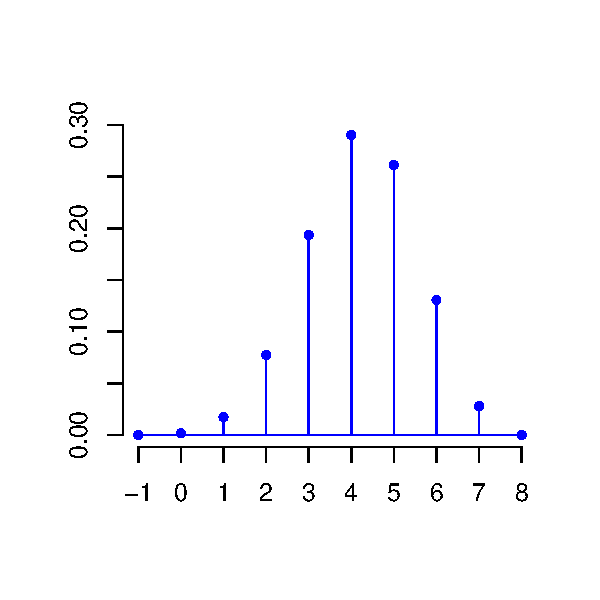
\includegraphics[scale=.5]{ch3_pmf6.pdf}&
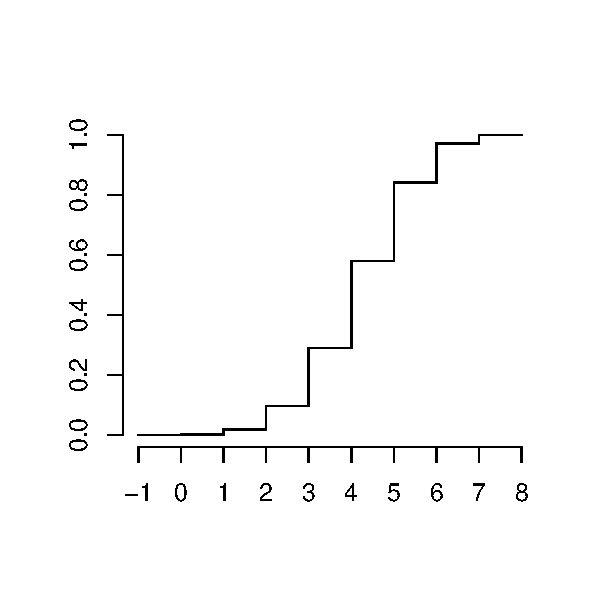
\includegraphics[scale=.5]{ch3_cdf.pdf}
\end{tabular}
\end{frame}


\begin{frame}{Properties of Variance}
\begin{block}{}
Let $X$ and $Y$ be random variables, and let $c$ be a constant. Then
\begin{enumerate}
\item $V(c) = 0$
\item $V(cX) = c^2V(X)$
\item $V(X+c) = V(X)$
\item If $X$ and $Y$ are independent, $V(X+Y)=V(X)+V(Y)$.
\end{enumerate}
\end{block}

\pause Example: Let $X$ be the number of heads when tossing a fair coin three times, so $X=Y_1+Y_2+Y_3$ where $Y_1$, $Y_2$, and $Y_3$ are independent Bernoulli random variables with parameter $p=.5$. By our formula for the variance of a Bernoulli,
$$V(Y_i)=p(1-p)=.5(1-.5)=.25$$
\pause Therefore,

\vspace{-.8cm}
\begin{align*}
V(X)&=V(Y_1+Y_2+Y_3)\\
&=V(Y_1)+V(Y_2)+V(Y_3)\\
&=.25+.25+.25=.75
\end{align*}
\end{frame}


%\begin{frame}{Properties of Variance}
%\begin{block}{}
%\vspace{-.2cm}$$V(c) = 0$$
%\end{block}
%Proof: $V(c)=E(c^2)-[E(c)]^2 = c^2 - c^2 = 0$
%\pause \begin{block}{}
%\vspace{-.2cm}$$V(cX) = c^2V(X)$$
%\end{block}
%Proof: $\begin{aligned}[t]V(cX) &= E[(cX)^2]-[E(cX)]^2 \\
%\uncover<3->{&= E[c^2X^2]-[cE(X)]^2 \\}
%\uncover<4->{&= c^2E(X^2)-c^2[E(X)]^2 \\}
%\uncover<5->{&= c^2[E(X^2)-[E(X)]^2] = c^2V(X)}
%\end{aligned}$
%\end{frame}
%
%\begin{frame}{Properties of Variance}
%\begin{block}{}
%If $X$ and $Y$ are independent, $V(X+Y)=V(X)+V(Y)$.
%\end{block}
%\pause Proof:
%\begin{align*}
%&V(X+Y) \\
%&= E[(X+Y)^2]-[E(X+Y)]^2 \\
%\uncover<3->{&=E(X^2+2XY+Y^2)-[E(X)+E(Y)]^2 \\}
%\uncover<4->{&= E(X^2)+2E(X)E(Y)+E(Y^2) - [E(X)]^2-2E(X)E(Y)-[E(Y)]^2 \\}
%\uncover<5->{&= E(X^2)-[E(X)]^2 + E(Y^2)-[E(Y)]^2 \\}
%\uncover<6->{&= V(X)+V(Y)}
%\end{align*}
%\end{frame}

\begin{frame}{Mean and Variance of Binomial Random Variables}
\begin{block}{}
A binomial random variable $X \sim \Bin(n,p)$ has mean and variance $E(X)=np$ and $V(X)=np(1-p)$. 
\end{block}
\pause Proof: Write $X$ as $X=Y_1+Y_2+\cdots+Y_n$
where $Y_1,\dots, Y_n$ are independent Bernoulli random variables with parameter $p$. Then
\begin{align*}
E(Y_i)= p, \quad V(Y_i)= p(1-p)
\end{align*}
\pause Therefore,
\begin{align*}
E(X)&=E(Y_1+\cdots+Y_n)\\
&=E(Y_1)+\cdots+E(Y_n)\\
&= p+\cdots+p = np \\[.5cm]
\uncover<3->{V(X)&=V(Y_1+\cdots+Y_n)\\
&=V(Y_1)+\cdots+V(Y_n)\\
&= p(1-p)+\cdots+p(1-p) = np(1-p)}
\end{align*}
%\begin{align*}
%E(X) &= \sum_{x=0}^{n} x\cdot f(x) \\
%&=\sum_{x=0}^n x\binom n x p^x(1-p)^{n-x} \\
%&= \sum_{x=0}^n x\frac{n!}{x!(n-x)!} p^x(1-p)^{n-x}
%\end{align*}
\end{frame}
%

%\begin{frame}{Quiz}
%Next class we'll have a quiz. I'll describe a couple of discrete random variables and ask you to find their pmf, expected value, and variance. One of these will be a binomial random variable.
%
%\vspace{.2cm}
%See Practice Quiz 2 posted on Canvas.
%\end{frame}



\begin{frame}{Problem}
\begin{block}{}A manufacturer produces widgets which work with probability $.4$. Suppose we test widgets one at a time until we find one that works. Let $X$ be the number of bad widgets we try before we find one that works. What is the probability that $X=2$?
\end{block}

\pause Solution: Let $Y_i$ be the Bernoulli random variable representing whether the $i$th widget works. Saying $X=2$ is the same as saying $Y_1=0, Y_2=0, Y_3=1$. Therefore,
\begin{align*}
P(X=2) &= P(Y_1=0, Y_2=0, Y_3=1) \\
&= P(Y_1=0)P(Y_2=0)P(Y_3=1) \\
&= (.6)(.6)(.4) = .144
\end{align*}
\end{frame}

\begin{frame}{Geometric Random Variable}
Suppose we have a sequence of independent trials each with probability $p$ of success. Let $X$ be the number of failures before the first success. The possible values of $X$ are 0, 1, 2, \dots 
We say that $X$ is a \emph{geometric random variable} with parameter $p$.

\begin{block}{}
The pmf of a geometric random variable with parameter $p$ is $f(x)=p(1-p)^x$.
\end{block}

\pause \vspace{.2cm}
Proof: We may model the trials as a sequence of independent Bernoulli random variables $Y_1, Y_2, \dots$ each with parameter $p$. Then we can calculate the pmf of $X$:
\begin{align*}
P(X=x)&=P(Y_1=0, Y_2=0, \dots, Y_x=0, Y_{x+1}=1)\\
&= P(Y_1=0)P(Y_2=0)\cdots P(Y_x=0)P(Y_{x+1}=1)\\
&= (1-p)^xp
\end{align*}
\end{frame}

\begin{frame}{Example}
\begin{block}{}A manufacturer produces widgets which work with probability $.4$. Suppose we test widgets one at a time until we find one that works. Let $X$ be the number of bad widgets we try before we find one that works. What is the pmf of $X$?
\end{block}

\pause
The pmf of a geometric random variable is $f(x)=p(1-p)^x$. In this case, $p=.4$, so this becomes $f(x)=.4(.6)^x$.

\vspace{-1cm}
\begin{center}
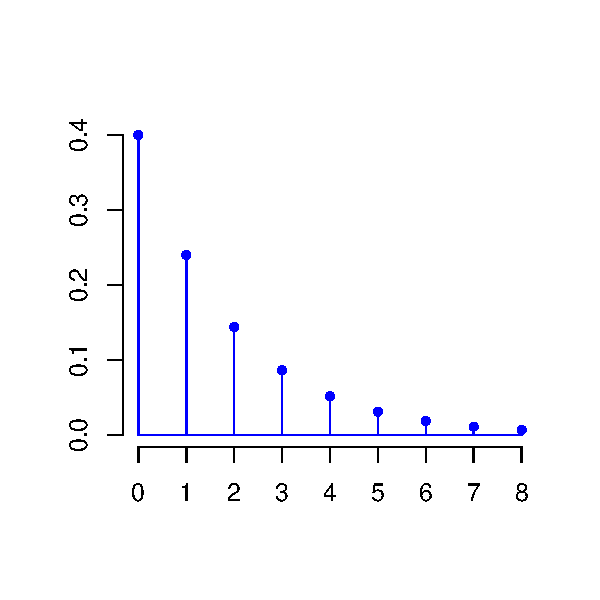
\includegraphics[scale=.6]{ch3_pmf4.pdf}
\end{center}

\end{frame}

\begin{frame}{Geometric Sums}
\begin{block}{}
Let $r\neq 1$ be a real number. Then
$$\sum_{j=0}^n r^j = 1+r+r^2+\cdots+r^n = \frac{1-r^{n+1}}{1-r}$$
\end{block}
\pause Example: $\begin{aligned}[t]1+\frac12+\left(\frac12\right)^2+\cdots+\left(\frac12\right)^5 
&= \frac{1-(1/2)^6}{1-1/2}\\
&= \frac{\frac{63}{64}}{1/2} = \frac{63}{32} \end{aligned}$

\pause Proof:
\begin{align*}
(1-r)(1+r+r^2+\cdots+r^n) & = 1+r+r^2+\cdots+r^n \\
&\quad -(r+r^2+\cdots+r^n+r^{n+1}) \\
&= 1-r^{n+1}
\end{align*}
Now divide by $1-r$.
\end{frame}

\begin{frame}{Infinite Geometric Sums}

\begin{block}{}
Let $r$ be a real number with $|r|<1$. Then $$\sum_{j=0}^\infty r^j = \frac1{1-r}$$
\end{block}

\pause Proof: 
\vspace{-0.6cm}
\begin{align*}
\sum_{j=0}^\infty r^j &= 1+r+r^2+\cdots 
= \lim_{n\to\infty} \sum_{j=0}^n r^j \\
&= \lim_{n\to\infty} \frac{1-r^{n+1}}{1-r} 
= \frac 1{1-r}
\end{align*}

\pause\vspace{.5cm} Example: 

\vspace{-1cm}
\begin{align*}
\sum_{j=0}^\infty \left(\frac12\right)^j &= 1 + \frac12 + \frac14 + \frac18 + \dots \\
&= \frac1{1-\frac12} = 2
\end{align*}
\end{frame}

\begin{frame}{Sum of PMF of Geometric Random Variable}
\pause If $f(x)$ is the pmf of a geometric random variable, we can confirm that the values of $f(x)$ add up to 1 (as they must for any pmf), using the formula $\sum_{j=0}^\infty r^j = \frac1{1-r}$ from the previous slide:
\begin{align*}
\sum_{x=0}^\infty f(x) &= \sum_{x=0}^\infty p(1-p)^{x} \\
\uncover<3->{&=p\sum_{x=0}^\infty (1-p)^x \\}
\uncover<4->{&= p\cdot \frac1{1-(1-p)}} \uncover<5->{ = p\cdot \frac1p = 1}
\end{align*}
%\uncover<6->{This confirms that $f(x)=(1-p)^{x-1}p$ is a valid pmf.}
\end{frame}

\begin{frame}{CDF of Geometric Distribution}
\begin{block}{}
The cdf of a geometric random variable $X$ with parameter $p$ is $F(x)=1-(1-p)^{x+1}$.
\end{block}
\pause 
Proof: For any integer $t \geq 0$, we calculate
\begin{align*}
F(t) = P(X \leq t) &= \sum_{x=0}^t P(X=x)\\
\uncover<3->{&= \sum_{x=0}^t p(1-p)^x \\}
\uncover<4->{&= p\sum_{x=0}^t (1-p)^x \\}
\uncover<5->{&= p\cdot \frac{1 - (1-p)^{t+1}}{1-(1-p)} \\}
\uncover<6->{&= 1-(1-p)^{t+1}}
\end{align*}
%\uncover<7->{for integers $x\geq0$.}
\end{frame}

\begin{frame}{CDF of Geometric Distribution}
Alternate proof: The event $X \leq x$ means that there are no more than $x$ failures before the first success, which is the same as saying that a success occurs among the first $x+1$ trials:
\pause 
\begin{align*}
P(X \leq x) &= P(Y_1=1 \cup Y_2=1 \cup \cdots \cup Y_{x+1}=1) \\
&= 1-P(Y_1=0 \cap Y_2=0 \cap \cdots \cap Y_{x+1}=0) \\
&= 1- P(Y_1=0)P(Y_2=0)\cdots P(Y_{x+1}=0) \\
&= 1- (1-p)^{x+1}
\end{align*}

\pause Example: Here is a graph of the cdf for $p=.4$:
%\begin{tabular}{p{4.5cm}p{4.5cm}}
%\vspace{-.6cm}
%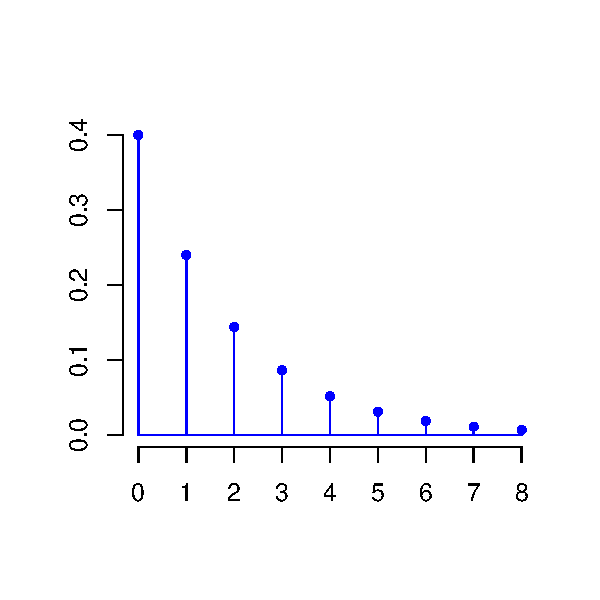
\includegraphics[scale=.5]{ch3_pmf4.pdf}
%&
%\vspace{-.6cm}
\vspace{-0.7cm}
\begin{center}
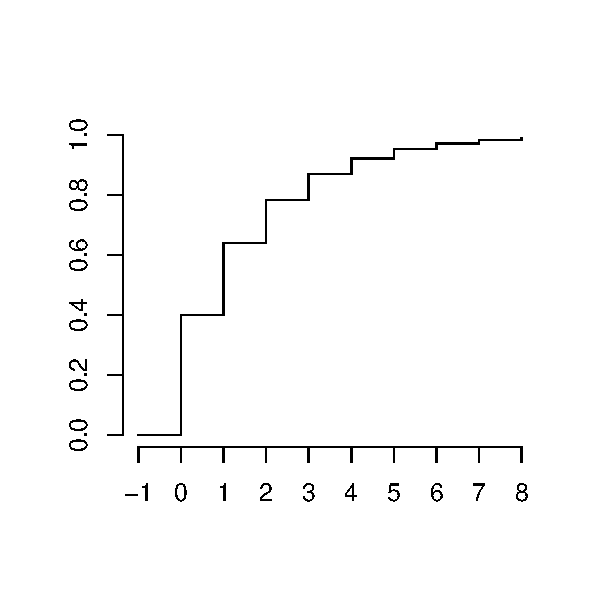
\includegraphics[scale=.48]{ch3_cdf_geom.pdf}
\end{center}
%\end{tabular}
\end{frame}

\begin{frame}{Mean of Geometric Distribution}
We can use calculus to find the mean of a geometric random variable $X$:
\vspace{-.2cm}
\pause \begin{align*}
E(X) &= \sum x\cdot f(x) = \sum_{x=0}^\infty xp(1-p)^x \\
\uncover<3->{&= p(1-p) \sum_{x=0}^\infty x(1-p)^{x-1} \\}
\uncover<4->{&= -p(1-p)
\sum_{x=0}^\infty \frac{d}{dp} (1-p)^x \\}
\uncover<5->{&= -p(1-p)\frac{d}{dp} \sum_{x=0}^\infty (1-p)^x \\}
\uncover<6->{&= -p(1-p)\frac{d}{dp} \frac1{1-(1-p)}\\}
\uncover<7->{&= -p(1-p)\frac{d}{dp} \frac1p }
\uncover<8->{= -p(1-p)\cdot\frac{-1}{p^2} = \frac1p-1}
%\sum_{x=1}\infty -(1-p)^xp
\end{align*}
\end{frame}

\begin{frame}{Example}
\begin{tabular}{@{}p{7.6cm}p{3.5cm}}
\vspace{0cm}
If we roll 5 six-sided dice at once, and all the dice turn up the same number, this is called a ``Yahtzee". The probability of getting a Yahtzee is $1/6^4=1/1296$. If we keep rolling 5 dice until we get a Yahtzee, what is the expected value of the number of times that we must try?
%\pause
%Recall that if we draw 2 cards from a standard deck of 52 cards, the probability that both will be aces is $\frac{4}{52}\cdot \frac{3}{51} = \frac1{221}$. Suppose we repeatedly shuffle the deck and draw two cards. What is the expected number of attempts until both cards are aces?
&
\vspace{0cm}
\includegraphics[scale=.25]{yahtzee.jpg}
\end{tabular}

\vspace{.3cm}
\pause \textbf{Solution}: The number of failures $X$ until we succeed is a geometric random variable with parameter $p=1/1296$. We calculate
$$E(X)=\frac1p - 1 = \frac1{1/1296}-1 = 1296-1 = 1295$$
\pause Now, the number of tries until we succeed is $X+1$, which has expected value
$$E(X+1) = E(X)+1 = 1295+1 = 1296$$
\end{frame}

\begin{frame}{Variance of Geometric Distribution}
By a similar technique, we can find the variance:
\pause{\small \begin{align*}
E(X^2) &= \sum x^2\cdot f(x) = \sum_{x=0}^\infty x^2p(1-p)^x \\
\uncover<3->{&= -p(1-p)\frac{d}{dp}\sum_{x=0}^\infty x(1-p)^x \\}
\uncover<4->{&= -p(1-p)\frac{d}{dp}(1-p)\frac{d}{dp}\sum_{x=0}^\infty (1-p)^x \\}
\uncover<5->{&= p(1-p)\frac{d}{dp}(1-p)\frac{d}{dp}\frac1p }
\uncover<6->{= p(1-p)\frac{d}{dp}(1-p)\left(\frac{-1}{p^2}\right)\\}
\uncover<7->{&= p(1-p)\frac{d}{dp}\left(\frac{-1}{p^2}+\frac1{p}\right)}
\uncover<8->{=
1-\frac3p+\frac2{p^2}\\[.1cm]}
%\frac{(1-p)(2-p)}{p^2}
%(p-1)(\frac2{p^2}-\frac1p)
%\end{align*}}
%\begin{align*}
\uncover<8->{
V(X)&=E(X^2)-[E(X)]^2 \\}
\uncover<9->{
&= 1-\frac3p+\frac2{p^2} - \left(\frac1p-1\right)^2 = \frac1{p^2}-\frac1p}
\end{align*}}
\end{frame}

\begin{frame}{Problem}
\begin{block}{}A manufacturer produces widgets which work with probability $.8$. Suppose we test widgets one at a time. Let $X$ be the number of bad widgets we test until we find 5 that work. What is the probability that $X=2$?
\end{block}

\pause \textbf{Solution}: Let $Y_i$ be the Bernoulli random variable representing whether the $i$th widget works. Saying $X=2$ is the same as saying that we have 2 failures before our 5th success, meaning our 5th success occurs on the 7th trial. \pause This means the 7th trial is a success, and there are 4 successes up through the 6th trial. \pause In other words, $Y_7=1$ and $Y_1+\cdots+Y_6=4$. \pause Now, $Y_1+\cdots+Y_6$ has a binomial distribution with parameters $n=6$ and $p=.8$. \pause Therefore
\begin{align*}
P(X=7) &= P(Y_1+\cdots +Y_6=4 \cap  Y_7=1) \\
\uncover<7->{&= P(Y_1+\cdots +Y_6=4)P(Y_7=1) \\}
\uncover<8->{&= \binom 6 4(.8)^4(.2)^2\cdot .8}
\uncover<9->{ \approx .197}
\end{align*}
\end{frame}

\begin{frame}{Negative Binomial Distribution}
Recall that a binomial random variable $X$ counts the number of successes out of a fixed number $n$ of independent trials. In contrast, a \emph{negative binomial} random variable $X$ counts the number of failures before we achieve a fixed number $r$ of successes. The possible values of $X$ are $0, 1, 2, \dots$.

\pause\vspace{.3cm} In the last slide we saw an example of a negative binomial random variable with $r=5$ and $p=.8$. In the same way we can write down the pmf of a general negative binomial random variable:
$$P(X=x)=\binom{x+r-1}{r-1} p^r(1-p)^x$$

\pause A geometric random variable is simply a negative binomial random variable with $r=1$. 
\end{frame}

\begin{frame}{Negative Binomial as Sum of Geometric}
A negative binomial random variable $X$ counts the number of failures it takes to get $r$ successes, given that the trials are independent and each have probability $p$ of success. 

\pause\vspace{.2cm}
The number of failures before the first success is a geometric random variable $Y_1$ with parameter $p$. 

\pause\vspace{.2cm}
After the first success, the number of additional failures until the next success is an independent geometric random variable $Y_2$. 

\pause\vspace{.2cm}
After $k$ successes, the number of additional failures until the next success is an independent geometric random variable $Y_{k+1}$. 

\pause\vspace{.2cm}
Therefore, we can express a negative binomial random variable $X$ as a sum of $r$ independent geometric random variables:
$$X=Y_1+\cdots+Y_r$$
\end{frame}

\begin{frame}{Mean and Variance of Negative Binomial}
Expressing a negative binomial random variable $X$ as a sum of independent geometric random variables allows us to compute its mean and variance. 
$$X=Y_1+\cdots+Y_r$$
\pause We know the mean and variance of geometric random variables:
\begin{align*}
E(Y_i) &= \frac1p-1 \\
V(Y_i) &= \frac1{p^2}-\frac1p
\end{align*}
\pause Therefore the mean and variance of $X=Y_1+\cdots+Y_n$ is
\begin{align*}
E(X) &= E(Y_1)+\dots+E(Y_r) = r\left(\frac1p-1\right) \\
V(X) &= V(Y_1)+\dots+V(Y_r) = r\left(\frac1{p^2}-\frac1p\right)
\end{align*}
\end{frame}

%\begin{frame}{Conflicting Definitions of Geometric and Negative Binomial}
%Given a sequence of independent trials each with probability $p$ of success, we defined a geometric random variable $X$ as the number of trials until the first success. The possible values are $1, 2, 3, \dots$.
%
%\pause\vspace{.2cm}
%However, we may also consider the \emph{shifted geometric} random variable $Y=X-1$ which counts the number of \textit{failures} before the first success. The possible values of $Y$ are 0, 1, 2, \dots.  Some authors (including Devore) call this a geometric random variable.
%
%\pause\vspace{.2cm}
%Similarly, while we defined the negative binomial as the number of \textit{trials} until the $r$th success, some authors define it instead as the number of \textit{failures} before the $r$th success.
%\end{frame}

\begin{frame}{Another Counting Problem}
\begin{block}{}
Suppose a bag contains 5 red balls and 7 green balls. If we draw 4 balls at random, what is the probability that exactly 2 are red?
\end{block}

\pause Solution:
\begin{itemize}
\pause \item There are $\binom{12}4=495$ ways to choose 4 balls from the 12 balls in the bag. Each of these 495 outcomes is equally likely. 
\pause \item Drawing exactly 2 red balls means that the remaining 2 balls drawn are green.
\pause \item The number of ways to choose 2 of 5 red balls is $\binom 5 2= 10$.
\pause \item The number of ways to choose 2 of 7 green balls is $\binom 7 2=21$.
\pause \item So the total number of ways to choose 2 red balls and 2 green balls is $10 \cdot 21= 210$. 
\pause \item The probability that this occurs is therefore $\frac{210}{495} = 42/99$.
\end{itemize}
\end{frame}

\begin{frame}{Hypergeometric Distribution}
\begin{block}{}
In general if we select $n$ individuals at random from a population of size $N$, where $M$ individuals are of type A, and $N-M$ are of type B, then the number $X$ of selected individuals of type A is a \emph{hypergeometric} random variable:
$$P(X=x)=\frac{\binom{M}x\binom{N-M}{n-x}}{\binom N n}$$
\end{block}
\pause Example: Suppose that out of a batch of 10 widgets, 7 are defective. If we randomly select 3 of the 10 widgets for inspection, what is the probability that we will find exactly 1 defective?

\vspace{.2cm}
\pause Here $X$ is hypergeometric with $n=3$, $N=10$, $M=7$, so
$$P(X=1) = \frac{\binom 7 1\binom 3 2}{\binom{10}3} = \frac{7\cdot 3}{120} = 7/40$$
\end{frame}

\begin{frame}{Example -- Animal Tagging}
\begin{block}{}
Researchers catch and tag 5 animals of a species thought to be near extinction in a certain region. After the animals have mixed back into the population, 10 animals from the population are randomly selected. Let $X$ be the number of tagged animals out of these 10. If there are actually 25 animals of this type in the region, what is the probability that (a) $X=2$? (b) $X\leq 2$?
\end{block}

\pause \begin{align*}
P(X=2) &= \frac{\binom 5 2\binom{20}8}{\binom{25}{10}} \approx .385\\[.3cm]
\uncover<3->{P(X\leq 2) &= P(X=0)+P(X=1)+P(X=2) \\
&= \frac{\binom 5 0\binom{20}{10}}{\binom{25}{10}} +
\frac{\binom 5 1\binom{20}{9}}{\binom{25}{10}} +
\frac{\binom 5 2\binom{20}{8}}{\binom{25}{10}} \approx .699}
\end{align*}
\end{frame}


\begin{frame}{Sampling Without Replacement}
Suppose that out of a batch of 20 widgets, 5 are defective. If we randomly draw two widgets from the 20, we may represent the outcome using two Bernoulli random variables, $Y_1$ and $Y_2$, where $Y_1=1$ if the first widget drawn is defective, and $Y_2=1$ if the second widget drawn is defective.

\vspace{.2cm}\pause
However, $Y_1$ and $Y_2$ are dependent, because if the first widget drawn is defective, this reduces the probability that the second widget drawn will be defective:
\begin{align*}
&P(Y_1=1)=P(Y_2=1)=5/20=.25 \\
&P(Y_2=1 \mid Y_1=1) = 4/19 \approx .211
\end{align*}

\pause This situation is called \emph{sampling without replacement} because once a widget is drawn, it is removed from the batch and may not be drawn again. 
The total number of defective widgets drawn in this way, $X=Y_1+Y_2$, is a \textit{hypergeometric} random variable.
\end{frame}

\begin{frame}{Sampling With Replacement}
Again suppose that out of a batch of 20 widgets, 5 are defective. Now draw two widgets at random, but this time after drawing the first widget, return it to the batch before randomly choosing the second widget. Thus there is a chance that the same widget will be chosen twice. This is called \emph{sampling with replacement}.

\vspace{.2cm}\pause
In this case, the two Bernoulli random variables $Y_1$ and $Y_2$ are independent, and the total number of defective widgets drawn $X=Y_1+Y_2$ is a \textit{binomial} random variable with $n=2$ and $p=5/20=1/4$.

\vspace{.2cm}\pause
In this case, the size of the batch (20 widgets) is irrelevant. If it had been a batch of 2000 widgets with 500 defective, it would not change the distribution of $X$. All that matters in this case is the \textit{proportion} of defective widgets.
%\vspace{.2cm}\pause
\end{frame}

\begin{frame}{Relationship between Binomial and Hypergeometric}
If the size of the batch is very large (say, 10000 widgets) and only a few widgets are drawn, then it makes little difference whether we sample with or without replacement, because it is very unlikely that any widget would be chosen more than once anyway. In this case, the hypergeometric and binomial distributions are practically identical.

\vspace{.2cm}
\pause In mathematical terms, the pmf of a hypergeometric random variable approaches the pmf of a binomial random variable, in the limit as we increase the population size $N$ while keeping the same proportion $p=M/N$.
\end{frame}

\begin{frame}{Binomial as Limit of Hypergeometric}
Given a hypergeometric random variable $X$ with $M/N=p$ and $n$ held constant while $N\to\infty$,
{\small
\begin{align*}
&P(X=x) 
= \dfrac{\binom M x\binom{N-M}{n-x}}{\binom N n} \\
\uncover<2->{&= \dfrac{\dfrac{M(M-1)\cdots(M-x+1)}{x!}\cdot\dfrac{(N-M)\cdots(N-M-n+x+1)}{(n-x)!}}{\dfrac{N(N-1)\cdots(N-n+1)}{n!}} \\}
\uncover<3->{&= \frac{n!}{x!(n-x)!}\frac{M(M-1)\cdots(M-x+1)}{N(N-1)\cdots(N-x+1)} 
\cdot \frac{(N-M)\cdots(N-M-n+x+1)}{(N-x)\cdots(N-n+1)} \\}
\uncover<4->{&= \binom n x \frac{p(p-\frac1N)\cdots(p-\frac{x-1}N)}{1(1-\frac1N)\cdots(1-\frac{x-1}N)}
\cdot \frac{(1-p)\cdots(1-p-\frac{n-x-1}N)}{(1-\frac{x}N)\cdots(1-\frac{n-1}N)}\\}
\uncover<5->{&\to \binom n x p^x(1-p)^{n-x}}
\end{align*}}
\uncover<6->{This agrees with the pmf of a binomial, $\Bin(n,p)$.}
\end{frame}

\begin{frame}{Binomial as Limit of Hypergeometric}
If we draw 15 widgets from a population with 30\% defective, the number of defective units is a hypergeometric random variable, but if we increase the population size while keeping the same proportion defective, it approaches binomial.

\vspace{-.9cm}
\begin{center}
\animategraphics[width=7.5cm,height=7.5cm]{5}{ch3_hyp}{1}{28}
\end{center}
\end{frame}

\begin{frame}{Mean of Hypergeometric Distribution}
Given a population of size $N$, of which $M$ are type A, if we sample $n$ random individuals without replacement, then the number of type A individuals selected is a hypergeometric random variable $X$. 

\pause \vspace{.2cm}
We may express $X$ as the sum of Bernoulli random variables, $X=Y_1+\cdots+Y_n$, where $Y_i=1$ if the $i$th individual sampled is a success. Each draw has probability $M/N$ of being a success, so $E(Y_i)=M/N$. Therefore,
\begin{align*}
E(X)&=E(Y_1+\cdots+Y_n) \\
&=E(Y_1)+\cdots+E(Y_n) \\
&=\frac M N+\cdots \frac M N = n\cdot\frac{M}{N}
\end{align*}
\pause If we set $p=M/N$, the probability of success for each draw, then we may write $E(X)=np$; this is the same mean as a binomial, $\Bin(n,p)$.
\end{frame}

\begin{frame}{Variance of Hypergeometric Distribution}
Although a hypergeometric random variable $X$ is the sum of Bernoulli random variables, $X=Y_1+\cdots+Y_n$, the random variables $Y_1,\dots,Y_n$ are dependent. Therefore we \textit{cannot} find the variance of $X$ by simply summing the variances of $Y_1, \dots, Y_n$.

\vspace{.2cm}
\pause Later we will show that the variance of $X$ is
$$V(X)=\frac{N-n}{N-1}\cdot np(1-p)$$

\pause We call $\frac{N-n}{N-1}$ the \textit{finite population correction factor}. When the population size $N$ is large compared to the sample size $n$, the correction factor is approximately 1 and the variance is approximately $np(1-p)$, the variance of a binomial, $\Bin(n,p)$.
\end{frame}

\begin{frame}{Poisson Process}
Consider a process where events occur at random times, such as
\begin{itemize}
\item The arrival times of customers at a store
\item Clicks of a Geiger counter exposed to a radioactive material
\item Webpage requests on an internet server
\item Incoming calls to a customer service center
\end{itemize}
\pause Such a process is called a \emph{Poisson process} if the following assumptions hold:
\begin{enumerate}
\item The mean number of events which occur in a time interval of length $t$ is $\lambda t$, where $\lambda$ is a constant, called the \emph{rate} of the Poisson process.
\item Events occur only one at a time.
\item The number of events which occur in a time interval is independent of the number and timing of past events.
\end{enumerate}
\end{frame}

\begin{frame}{Poisson Distribution}
Given a Poisson process with rate $\lambda$, we want to find the pmf of the number of events $X$ which occur in the time interval $I=[0,t]$.

\pause \begin{itemize}[<+->]
\item By assumption (1), the mean of $X$ is $\mu=\lambda t$.
\item Divide the interval $[0,t]$ into equal-width subintervals $I_1, \dots, I_n$, each of length $t/n$.
%$$I_k = \left[k\cdot\frac t n, (k+1)\cdot\frac t n\right]$$
\item Let $X_k$ be the number of events which occur in the subinterval $I_k$, so $X=X_1+X_2+\cdots+X_n$. 
\item By assumption (1), $E(X_k)=\lambda\cdot \frac t n= \frac\mu n$. 
\item By assumption (2), if $n$ is large, then the probability of more than one event occuring in any given interval $I_k$ is very small. 
\item So we may approximate $X_k$ as a Bernoulli random variable with parameter $p=\frac{\mu}n$.
\item By assumption (3), the random variables $X_1,\dots, X_n$ are independent. Thus $X$ is approximately binomial, $\Bin(n,\frac \mu n)$.
\end{itemize}
\end{frame}

\begin{frame}{Poisson Distribution}
Recall from calculus that
$$\lim_{n\to\infty} \left(1+\frac{r}n\right)^n = e^r$$
\pause We use this to find the pmf of a Poisson random variable $X$. We argued that for large $n$, $X$ is approximately binomial, $\Bin(n,\frac{\mu}n)$, so
\pause\begin{align*}
P(X=x) &\approx \binom n x (\mu/n)^x(1-\mu/n)^{n-x} \\
\uncover<4->{&= \frac{n(n-1)\cdots(n-x+1)}{x!}(\mu/n)^x(1-\mu/n)^{n-x} \\}
\uncover<5->{&= \frac{n(n-1)\cdots(n-x+1)}{nn \cdots n}(1-\mu/n)^n(1-\mu/n)^{-x}\cdot \frac{\mu^x}{x!} \\}
\uncover<6->{&\to 1 \cdot e^{-\mu}\cdot 1\cdot \frac{\mu^x}{x!} \hspace{4cm} (\text{as }n\to\infty)\\}
\uncover<7->{&= \frac{e^{-\mu}\mu^x}{x!}}
\end{align*}
\end{frame}

\begin{frame}{Poisson Distribution}
\begin{block}{}
Given a Poisson process with rate $\lambda$, the number $X$ of events which occur in a time interval of length $t$ is a \emph{Poisson} random variable with mean $\mu=\lambda t$. The possible values of $X$ are $0, 1, 2,\dots$
$$P(X=x)=\frac{e^{-\mu}\mu^x}{x!}$$
\end{block}

\pause \vspace{.1cm} Example: Suppose that at a small store, customers arrive at an average rate of 6 per hour. What is the probability that during a given hour only 3 or fewer customers will arrive?

\pause \vspace{.3cm}Assuming a Poisson process,
\begin{align*}
P(X\leq 3) &= P(X=0)+P(X=1)+P(X=2)+P(X=3) \\
&= \frac{e^{-6}6^0}{0!} + \frac{e^{-6}6^1}{1!} + \frac{e^{-6}6^2}{2!} + \frac{e^{-6}6^3}{3!} \\
&= e^{-6} (1+6 + 18 + 36) = 61e^{-6} \approx .151
\end{align*}
\end{frame}

\begin{frame}{Example}
\begin{block}{}
Suppose that at random times a system suffers breakdowns requiring immediate repairs. If the system breaks down at a rate of once per year, what is the probability that the system will break down 3 or more times in one year?
\end{block}
\pause Solution: The given information suggests that the number $X$ of breakdowns in a year is a Poisson random variable with mean 1. 
\pause \begin{align*}
P(X \geq 3) &= 1 - P(X \leq 2) \\
&= 1 - P(X=0) - P(X=1)-P(X=2) \\
&= 1 - \frac{e^{-1}1^0}{0!} - \frac{e^{-1}1^1}{1!} - \frac{e^{-1}1^2}{2!} \\
&= 1 - e^{-1}\left(1+1+\frac12\right) \\
&= 1 - \frac{5e^{-1}}2 \approx .080
\end{align*}
\end{frame}

\begin{frame}{Poisson as Limit of Binomial Distribution}
Compare a $\Bin(n,6/n)$ with a Poisson with $\mu=6$:
%\begin{center}
%\flashmovie[width=6cm,height=6cm]{ch3_poi.swf}
%\flashmovie[engine=flv-player,auto=1,controlbar=0]{ch3_poi.flv}
%\movie[width=6cm,height=6cm,loop]{Hello}{ch3_poi.swf}
%\includemovie[ poster,  text={Blah}]{6cm}{6cm}{ch3_poi.swf}
%\end{center}
\vspace{-.8cm}
\begin{center}
\animategraphics[width=9cm,height=9cm]{5}{ch3_poi}{1}{33}
\end{center}
\end{frame}

\begin{frame}{Poisson Distribution}
Recall from calculus that
$$e^\mu=\sum_{x=0}^\infty \frac{\mu^x}{x!}$$
\pause Therefore, the pmf $f(x)$ of a Poisson random variable satisfies
\begin{align*}
\sum_{x=0}^\infty f(x) &= \sum_{x=0}^\infty \frac{e^{-\mu}\mu^x}{x!} \\
\uncover<3->{&= e^{-\mu} \sum_{x=0}^\infty \frac{\mu^x}{x!}\\}
\uncover<4->{&=e^{-\mu}e^\mu\\}
\uncover<5->{&=1}
\end{align*}
\uncover<6->{which shows that $f(x)$ is a valid pmf.}
\end{frame}

\begin{frame}{Mean of Poisson Distribution}
We may directly calculate the mean of a Poisson random variable $X$ based on the pmf:
\pause \begin{align*}
E(X) &= \sum_{x=0}^\infty x\cdot\frac{e^{-\mu}\mu^x}{x!} \\
\uncover<3->{&= \sum_{x=1}^\infty \frac{e^{-\mu}\mu^x}{(x-1)!} \\}
\uncover<4->{&= \sum_{x=0}^\infty \frac{e^{-\mu}\mu^{x+1}}{x!} \\}
\uncover<5->{&= \mu \sum_{x=0}^\infty \frac{e^{-\mu}\mu^x}{x!} \\}
\uncover<6->{&= \mu}
\end{align*}
\uncover<7->{This is what we expected based on the definition.}
\end{frame}

\renewcommand{\arraystretch}{1.35}
%\setlength{\extrarowheight}{.5cm}

\begin{frame}{Variance of Poisson Distribution}
We can also calculate the variance:
{\small
\pause \begin{align*}
E(X^2) &= \sum_{x=0}^\infty x^2\cdot\frac{e^{-\mu}\mu^x}{x!}\\
\uncover<3->{&= \sum_{x=1}^\infty x\cdot\frac{e^{-\mu}\mu^x}{(x-1)!}\\}
\uncover<4->{&= \sum_{x=0}^\infty (x+1)\frac{e^{-\mu}\mu^{x+1}}{x!}\\}
\uncover<5->{&= \sum_{x=0}^\infty x\frac{e^{-\mu}\mu^{x+1}}{x!} + \sum_{x=0}^\infty \frac{e^{-\mu}\mu^{x+1}}{x!}\\}
\uncover<6->{&= \sum_{x=1}^\infty \frac{e^{-\mu}\mu^{x+1}}{(x-1)!} + \mu\sum_{x=0}^\infty \frac{e^{-\mu}\mu^{x}}{x!}\\}
%&= \sum_{x=1}^\infty \frac{e^{-\mu}\mu^{x+1}}{(x-1)!} + \mu
\uncover<7->{&= \sum_{x=0}^\infty \frac{e^{-\mu}\mu^{x+2}}{x!}+\mu}
\uncover<8->{= \mu^2+\mu}
%\uncover<4->{&= \sum_{x=1}^\infty ((x-1)+1)\cdot\frac{e^{-\mu}\mu^x}{(x-1)!}\\}
%\uncover<5->{&= \sum_{x=1}^\infty (x-1)\cdot\frac{e^{-\mu}\mu^x}{(x-1)!}+ \sum_{x=1}^\infty \frac{e^{-\mu}\mu^x}{(x-1)!}\\}
%\uncover<6->{&= \mu^2\sum_{x=2}^\infty \frac{e^{-\mu}\mu^{x-2}}{(x-2)!}+ \mu\sum_{x=1}^\infty \frac{e^{-\mu}\mu^{x-1}}{(x-1)!}\\}
%\uncover<7->{&= \mu^2\sum_{x=0}^\infty \frac{e^{-\mu}\mu^x}{x!}+ \mu\sum_{x=0}^\infty \frac{e^{-\mu}\mu^x}{x!}=\mu^2+\mu}
\end{align*}}
\uncover<9->{So $V(X)=E(X^2)-[E(X)]^2=\mu^2+\mu-\mu^2 = \mu$.}
\end{frame}
%
%\begin{frame}{Infinite Mean}
%Recall from calculus that the series
%$$\sum_{x=1}^\infty \frac1{x^2} = 1+\frac14+\frac19+\frac1{16}+\cdots$$
%converges by the Integral Test. So if we let $c=\sum_{x=1}^\infty\frac1{x^2}$, then
%$$f(x)=\frac{c^{-1}}{x^2}$$
%defines a pmf for a random variable $X$. But
%\begin{tabular}{p{5.7cm}p{5cm}}
%\vspace{0cm}
%$\begin{aligned}[t]E(X)&=\sum_{x=1}^\infty x\cdot f(x) = \sum_{x=1}^\infty x\cdot\frac{c^{-1}}{x^2} \\
%&= c^{-1} \sum_{x=1}^\infty \frac1x = \infty
%\end{aligned}$
%&
%\vspace{-1.2cm}
%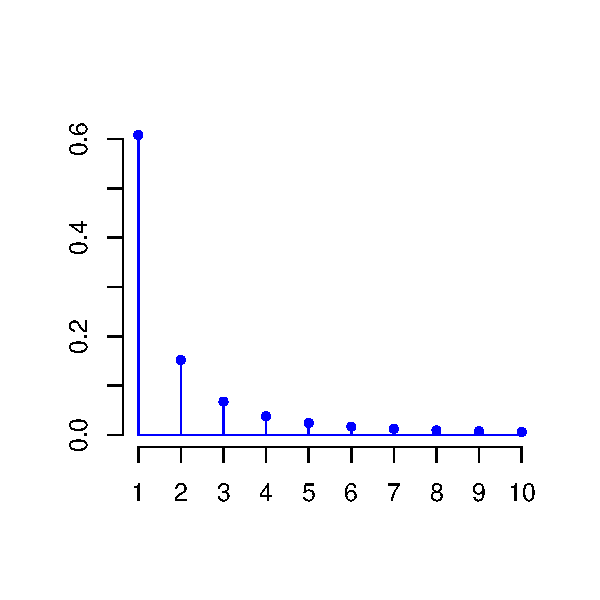
\includegraphics[scale=.55]{ch3_pmf_inf.pdf}
%\end{tabular}
%\end{frame}


\begin{frame}{Summary}
The \emph{probability mass function (pmf)} of a discrete random variable $X$ is
$$f(x) = P(X = x)$$
The \emph{cumulative distribution function (cdf)} is
$$F(x) = P(X \leq x)$$
A \emph{Bernoulli} random variable $X$ with parameter $p$ takes the value 1 with probability $p$ and the value 0 with probability $1-p$.

\vspace{.3cm}
The \emph{binomial coefficient} $\binom n k=\frac{n!}{k!(n-k)!}$
is the number of ways of choosing a subset of $k$ objects from a set of $n$ objects.
\end{frame}

\begin{frame}{Summary}
The \emph{expected value} or \emph{mean} of a discrete random variable $X$ is $E(X)=\sum x\cdot f(x)$.
\begin{block}{}
\begin{enumerate}
\item $E(c) = c$
\item $E(cX) = cE(X)$
\item $E(X+Y) = E(X)+E(Y)$
%\item If $X$ and $Y$ are independent, then $E(XY) = E(X)E(Y)$.
\end{enumerate}
\end{block}

The \emph{variance} is $V(X)=E[(X-\mu)^2]=E(X^2)-\mu^2$ where $\mu=E(X)$. The \emph{standard deviation} is $\sigma = \sqrt{V(X)}$.
\begin{block}{}
Let $X$ and $Y$ be random variables, and let $c$ be a constant. Then
\begin{enumerate}
\item $V(c) = 0$
\item $V(cX) = c^2V(X)$
\item $V(X+c) = V(X)$
\item If $X$ and $Y$ are independent, $V(X+Y)=V(X)+V(Y)$.
\end{enumerate}
\end{block}

\end{frame}

\begin{frame}{Summary}

\small
\hspace*{-1cm}\begin{tabular}{p{1.55cm}|p{3.25cm}|p{2.5cm}|p{1.2cm}|p{2.2cm}}
Distribution & Random variable $X$ & pmf & Mean & Variance\\ \hline
Binomial & Number of successes out of $n$ independent trials & \vspace{-.4cm}\begin{tabular}{@{}l}$\binom n x p^x(1-p)^{n-x}$ \\ \scriptsize $x=0, 1, \dots, n$\end{tabular} & $np$ & $np(1-p)$\\ \hline
Geometric & Number of failures until first success & \vspace{-.4cm}\begin{tabular}{@{}l} $p(1-p)^x$ \\[-.15cm] \scriptsize $x=0, 1, 2, \dots$ \end{tabular} & \vspace{-.25cm}$\frac1p-1$ & \vspace{-.25cm}$\displaystyle\frac1{p^2}-\frac1p$ \\ \hline
Negative Binomial & Number of failures until $r$ successes & \vspace{-.4cm}\begin{tabular}{@{}l} $\binom{x+r-1}{r-1}p^r(1-p)^x$ \\[-.15cm] \scriptsize $x=0, 1, 2, \dots$ \end{tabular} & \vspace{-.25cm}$r(\frac1p-1)$ & \vspace{-.28cm}$\displaystyle r\left(\frac1{p^2}-\frac1p\right)$\\ \hline
Hyper-geometric & Number of type A in a random sample of size $n$ from a population of size $N$ containing $M$ of type A & \vspace{-.15cm}\begin{tabular}{@{}l}$\displaystyle\frac{\binom M x\binom {N-M}{n-x}}{\binom N n}$ \\ \scriptsize $x=0,\dots,n$ \end{tabular}& \vspace{-.15cm}\begin{tabular}{@{}l}$np$ \\ where \\ $p=\frac M N$\end{tabular}& \vspace{-.2cm}$\frac{N-n}{N-1}\cdot np(1-p)$ \\ \hline
Poisson & Number of events occuring over an interval of time, where events occur at random times& \vspace{-.15cm}\begin{tabular}{@{}l}$\displaystyle \frac{e^{-\mu}\mu^x}{x!}$ \\ \scriptsize $x=0, 1, 2, \dots$ \end{tabular} & $\mu$ & $\mu$
\end{tabular}
\end{frame}

\end{document}
